% compress:
% gs -sDEVICE=pdfwrite -dCompatibilityLevel=1.4 -dNOPAUSE -dQUIET -dBATCH      -sOutputFile=CompressedSwarmControlIJRR.pdf SwarmControlIJRR.pdf
%%%%%%%%% IJRR SETTINGS
%  from https://us.sagepub.com/en-us/nam/manuscript-submission-guidelines#PreparingYourManuscript
%\documentclass[Afour,sageh,times]{sagej} % sage_latex_guidelines.tex V1.01, 11 June 2015
\documentclass[conference]{IEEEtran}
\IEEEoverridecommandlockouts% This command is only needed if 
                                                          % you want to use the \thanks command
%\overrideIEEEmargins                                      % Needed to meet printer requirements.
\usepackage{times}


\makeatletter 
\let\NAT@parse\undefined
\makeatother

% numbers option provides compact numerical references in the text. 
%\usepackage[numbers]{natbib}
\usepackage{multicol}
\usepackage[bookmarks=true]{hyperref}

\usepackage{bbm}
\usepackage{calc}
\usepackage{url}
\usepackage{transparent}
\usepackage{hyperref}
\hypersetup{
  colorlinks =false,
  urlcolor = black,
  linkcolor = black
}
\usepackage{graphicx}
\usepackage[cmex10]{amsmath}
\usepackage{bm}
\usepackage{amssymb}
\usepackage{rotating}

\usepackage{chngcntr}
\counterwithin{paragraph}{subsection} % makes paragraph depend on subsection


%\usepackage{xfrac}
\usepackage{nicefrac}
\usepackage{cite}
\usepackage[caption=false,font=footnotesize]{subfig}
\usepackage[usenames, dvipsnames]{color}
\usepackage{colortbl}
%\usepackage{caption}

%\usepackage{wrapfig}
\usepackage{overpic}
%\usepackage{subfigure}
%\usepackage{textcomp}
\graphicspath{{./pictures/pdf/},{./pictures/ps/},{./pictures/png/},{./pictures/jpg/}}
\usepackage{breqn} %for breaking equations automatically
\usepackage[ruled]{algorithm}
\usepackage{algpseudocode}
%\usepackage{algorithmic}
\usepackage{multirow}
\usepackage{todonotes}
\usepackage{authblk}

%\newcommand{\todo}[1]{\vspace{5 mm}\par \noindent \framebox{\begin{minipage}[c]{0.98 \columnwidth} \ttfamily\flushleft \textcolor{red}{#1}\end{minipage}}\vspace{5 mm}\par}
% uncomment this to hide all red todos
%\renewcommand{\todo}{}

%% ABBREVIATIONS
\newcommand{\qstart}{q_{\text{start}}}



%% MACROS


\providecommand{\abs}[1]{\left\lvert#1\right\rvert}
\providecommand{\norm}[1]{\left\lVert#1\right\rVert}
\providecommand{\normn}[2]{\left\lVert#1\right\rVert_#2}
\providecommand{\dualnorm}[1]{\norm{#1}_\ast}
\providecommand{\dualnormn}[2]{\norm{#1}_{#2\ast}}
\providecommand{\set}[1]{\lbrace\,#1\,\rbrace}
\providecommand{\cset}[2]{\lbrace\,{#1}\nobreak\mid\nobreak{#2}\,\rbrace}
\providecommand{\lscal}{<}
\providecommand{\gscal}{>}
\providecommand{\lvect}{\prec}
\providecommand{\gvect}{\succ}
\providecommand{\leqscal}{\leq}
\providecommand{\geqscal}{\geq}
\providecommand{\leqvect}{\preceq}
\providecommand{\geqvect}{\succeq}
\providecommand{\onevect}{\mathbf{1}}
\providecommand{\zerovect}{\mathbf{0}}
\providecommand{\field}[1]{\mathbb{#1}}
\providecommand{\C}{\field{C}}
\providecommand{\R}{\field{R}}
\newcommand{\Cspace}{\mathcal{Q}}
\newcommand{\Uspace}{\mathcal{U}}
\providecommand{\Fspace}{\Cspace_\text{free}}
\providecommand{\Hcal}{$\mathcal{H}$}
\providecommand{\Vcal}{$\mathcal{V}$}
\DeclareMathOperator{\conv}{conv}
\DeclareMathOperator{\cone}{cone}
\DeclareMathOperator{\homog}{homog}
\DeclareMathOperator{\domain}{dom}
\DeclareMathOperator{\range}{range}
\DeclareMathOperator{\sign}{sgn}
\providecommand{\polar}{\triangle}
\providecommand{\ainner}{\underline{a}}
\providecommand{\aouter}{\overline{a}}
\providecommand{\binner}{\underline{b}}
\providecommand{\bouter}{\overline{b}}
\newcommand{\D}{\nobreakdash-\textsc{d}}
%\newcommand{\Fspace}{\mathcal{F}}
\providecommand{\Fspace}{\Cspace_\text{free}}
\providecommand{\free}{\text{\{}\mathsf{free}\text{\}}}
\providecommand{\iff}{\Leftrightarrow}
\providecommand{\subinner}[1]{#1_{\text{inner}}}
\providecommand{\subouter}[1]{#1_{\text{outer}}}
\providecommand{\Ppoly}{\mathcal{X}}
\providecommand{\Pproj}{\mathcal{Y}}
\providecommand{\Pinner}{\subinner{\Pproj}}
\providecommand{\Pouter}{\subouter{\Pproj}}
\DeclareMathOperator{\argmax}{arg\,max}
\providecommand{\Aineq}{B}
\providecommand{\Aeq}{A}
\providecommand{\bineq}{u}
\providecommand{\beq}{t}
\DeclareMathOperator{\area}{area}
\newcommand{\contact}[1]{\Cspace_{#1}}
\newcommand{\feasible}[1]{\Fspace_{#1}}
\newcommand{\dd}{\; \mathrm{d}}
\newcommand{\figwid}{0.22\columnwidth}
\newcommand{\TRUE}{\textbf{true}}
\newcommand{\FALSE}{\textbf{false}}
\DeclareMathOperator{\atan2}{atan2}
\allowdisplaybreaks

\newtheorem{theorem}{Theorem}
\newtheorem{definition}[theorem]{Definition}
\newtheorem{lemma}[theorem]{Lemma}


%useful for highlighting sections that need work
%\newcommand{\todo}[1]{\textcolor{red}{\footnotesize \textsf{#1}}}


%\setcounter{secnumdepth}{3}
%\runninghead{Shahrokhi \textit{et~al.}}
%\hyphenation{micro-robot nano-robot nano-robotics micro-robotics micro-robots nano-robots micro-manip-ulators}
%%%%%%%%%%%% For debugging purposes, I like to display the TOC
%    \tableofcontents
%    \setcounter{tocdepth}{3}
%    \newpage
%%%% END TOC %%%%%%%%%%%%%%%%%%%%%%%%%%%%%%%%%%%%%%%
 

\title{\LARGE \bf Steering a Swarm Using Global Inputs\\ and Swarm Statistics}


\author{Shiva Shahrokhi, Chris Ertel, Mable Wan, Lillian Lin, Aaron T. Becker% end author block 
\thanks{Authors are with the Department of Electrical and Computer Engineering,  University of Houston, Houston, TX 77204 USA        {\tt\small  \{sshahrokhi2, atbecker\}@uh.edu}}
}

\begin{document}

\maketitle
\thispagestyle{empty}
\pagestyle{empty}
\begin{abstract}
Microrobotics has the potential to revolutionize many applications including targeted material delivery, assembly, and surgery.  The same properties that promise breakthrough solutions---small size and large populations---present unique challenges for controlling motion. We want to use large swarms of particles to perform manipulation tasks; unfortunately, human-swarm interaction studies as conducted today are limited in sample size, are difficult to reproduce, and are prone to hardware failures. We present an alternative.

This paper first examines the perils, pitfalls, and possibilities we discovered by launching \href{http://www.swarmcontrol.net}{SwarmControl.net}, an online game where players steer swarms of up to 500 particles to complete manipulation challenges. We record statistics from thousands of players, and use the game to explore aspects of large-population particle control. We present the game framework as a new, open-source tool for large-scale user experiments. One surprising result was that humans completed an object manipulation task \emph{faster} when provided with only the mean and variance of the swarm than with full-state feedback. Inspired by human operators, this paper next investigates controllers that use only the mean and variance of the swarm. We prove that the mean position is controllable, then provide conditions under which variance is controllable.  We next derive automatic controllers for these and a hysteresis-based switching control to regulate the first two moments of the particle distribution.  Finally, we employ these controllers as primitives for an object manipulation task and implement all the automatic controllers on 100 kilobots controlled by the direction of a global light source.
\end{abstract}

%\keywords{micro-robot, global control, swarm, human-swarm interaction}




%\input{00-Abstract.tex}
\section{Introduction}\label{sec:Intro}
%This project studies system models and user interfaces for five multi-robot manipulation tasks with large populations of micro- and nanorobots.  We test several system models with different limitations on controllability and observability of the motion controller, and evaluate several different user interfaces.  We conduct user experiments to understand the impact of these limitations and design choices. 


%Micro- and nanorobotics have the potential to revolutionize many applications including targeted material delivery, assembly, and surgery.  The same properties that promise breakthrough solutions---small size and large populations---present unique challenges to generating controlled motion.  
Large populations of micro- and nanorobots are being produced in laboratories around the world, with diverse potential applications in drug delivery and construction, see \cite{Peyer2013,Shirai2005,Chiang2011}. These activities require robots that behave intelligently.
Limited computation and communication at small scales makes autonomous operation or direct control over individual robots difficult. 
Instead, this paper treats the robots as particles that are steered by a global control signal broadcast to the entire population.    
This paper examines object manipulation by a swarm of particles, as illustrated in Fig.~{\ref{fig:bigPictureMeanAndVarianceForSwarm}. 
The transportation methodology is similar to that in Sugawara's work \cite{sugawara2014object}, but rather than using onboard computation or sensing, the particles all move in the same direction.


%%%% Move it to the cover letter.
%This paper combines the content of two preliminary conference papers, extending their substance and providing full details in a single journal paper.
 % \cite{swarmcontrol2013} covered the first three months of SwarmControl.net experiments, and \cite{ShahrokhiIROS2015} presented simulations of object manipulation.  This paper presents three years of results from new games at SwarmControl.net.  For object manipulation, this paper presents robust new algorithms for manipulation, path planning, and obstacle avoidance, and a rich set of parametric studies.  All hardware validation experiments are new.

Many promising applications for particle swarms require direct human control, but user interfaces to thousands---or millions---of particles is a daunting human-swarm interaction (HSI) challenge. Our early work with over a hundred hardware robots and thousands of simulated particles demonstrated that direct human control of large swarms is possible, \cite{Becker2013b}. 
Unfortunately, the logistical challenges of repeated experiments with over one hundred robots prevented large-scale tests. 
There is currently no comprehensive understanding of user interfaces for controlling multi-robot systems with massive populations.  
One contribution of this paper is a tool for investigating HSI methods through statistically significant numbers of experiments.  


\begin{figure}
\centering
\begin{overpic}[width=\columnwidth]{MainExpFig.pdf}\end{overpic}
\caption{\label{fig:bigPictureMeanAndVarianceForSwarm} 
A swarm of particles, all actuated by a uniform control input where each particle gets the same control input, can be effectively manipulated by a control law that uses only the mean and variance of the robot distribution.  
Here a swarm of particles (kilobot robots) pushes a green hexagon toward the goal (see video attachment).
}
\end{figure}



%Inspired by our online experiments, because it is not always possible to gather pose information on each robot for feedback control and
%It is not always practical to gather pose information on individual robots for feedback control; the robots might be difficult or impossible to sense individually due to their size and location. However, it is often possible to sense global properties of the group, such as mean position and density.
Often particles are difficult or impossible to sense individually due to their size and location. 
For example, microrobots are smaller than the minimum resolution of a clinical MRI-scanner, see Martel \cite{martel2014computer}, however it is often possible to sense global properties of the group such as mean position and variance. 
To make progress in automatic control with global inputs, this paper presents swarm manipulation controllers inspired by our online experiments that require only mean and variance measurements of the particle's positions. 
 To perform the object manipulation task illustrated in Fig.~\ref{fig:bigPictureMeanAndVarianceForSwarm}, we use these controllers   as primitives, policy iteration for path planning, handle outliers by partitioning the workspace, and minimize pushing the object backwards with potential field navigation.


 %function and implementation function

 Our paper is organized as follows.  After a discussion of related work in \S \ref{sec:RelatedWork},  we describe our experimental methods for an online human-user experiment and their results in \S \ref{sec:expMethods}. Next we prove that the mean and variance of a particle swarm are controllable in \S \ref{sec:theory}, and present automatic controllers in \S \ref{sec:simulation}. We use these controllers as primitives and present a framework for manipulating an object through a maze in \S \ref{sec:exp}. 
 We conclude with implementations of these controllers in our hardware robots and use them to complete an object manipulation task with 100 kilobots in \S \ref{sec:realExperiment}.
 



%%%%%%%%%%%%%%%%%%%%%%%%%%%%%%%%%%%%%%%%%%%%%%%%%%%%%%%%%%%
\section{Related work}\label{sec:RelatedWork}
%%%%%%%%%%%%%%%%%%%%%%%%%%%%%%%%%%%%%%%%%%%%%%%%%%%%%%%%%%%

Controlling the \emph{shape}, or relative positions, of a swarm of robots is a key ability for a range of applications.  Correspondingly, it has been studied from a control-theoretic perspective in  both centralized and decentralized approaches. For examples of each, see the centralized virtual leaders in \cite{egerstedt2001formation}, and the  gradient-based decentralized controllers  using control-Lyapunov functions in~\cite{hsieh2008decentralized}. However, these approaches assume a level of intelligence and autonomy in individual robots that exceeds the capabilities of many systems, including current micro- and nano-robots.  Current micro- and nano-robots, such as those in~\cite{Chowdhury2015,martel2015magnetotactic,Xiaohui2015magnetiteMicroswimmers} lack onboard computation.

This chapter focuses on centralized techniques that apply the same control input to both particles. 
Precision control requires breaking the symmetry caused by the uniform input.  
Symmetry can be broken using particles that respond differently to the uniform control signal, either through agent-agent reactions \cite{bertozzi2015ring}, or engineered inhomogeneity  \cite{Donald2013,bretl2007,beckerIJRR2014}. 
 The magnetic gradients of MRI scanners are \emph{uniform}, meaning the same force is applied everywhere in the workspace\cite{nosrati2018development}.
 This work assumes a uniform control with homogenous particles, as in~\cite{AaronManipulation2013}, and breaks the control symmetry using obstacles in the workspace. 

%The techniques in this paper are inspired by artificial force-fields. 

%\emph{Fluid-flow:} 
%Fluid flow along boundaries generates a shear force that pushes different parts of a body in opposing directions. 
%Most introductory fluid dynamics textbooks provide models~\citep{Munson2013}.
%Similarly, a swarm of robots under global control pushed along a boundary will experience shear forces.  
%This is a position-dependent force, and so can be exploited to control the configuration or shape of the swarm.  
% \citep{spears2006physics}~used these forces to disperse a swarm's spatial position for coverage for physics-based swarm simulations.

%\emph{Artificial Force-fields:}
%Much research has focused on generating non-uniform artificial force-fields that can be used to rearrange passive components. 
Alternative techniques rely on non-uniform inputs, such as artificial force-fields.
Applications have included techniques to design shear forces for sensorless manipulation of a single object by~\cite{lamiraux+2001:ra}.  
\cite{vose2012sliding} demonstrated a collection of 2D force fields generated by six degree-of-freedom vibration inputs to a rigid plate.  These force fields, including shear forces, could be used as a set of primitives for motion control to steer the formation of multiple objects. %However unlike the uniform control model in this paper, their control was multi-modal and position-dependent.
%\todo{talk about obstacles, think about adding goldberg}

%This paper develops control algorithms using uniform control fields, such as the magnetic resonance navigation \cite{nosrati2018development}.%field in a clinical MRI [insert a recent reference from Sylvain Martel using MRI].
Similarly, much recent work in magnet control has focused on exploiting inhomogeneities in the magnetic field to control multiple micro particles  using gradient-based pulling~\cite{Salmanipour2018EightDOF,Denasi2018independent}.  
Unfortunately, using large-scale external magnetic fields makes it challenging to independently control more than one microrobot unless the  distance between the electromagnetic coils is at the same length scales as the robot workspace~\cite{diller2016six, Denasi2018independent, Salmanipour2018EightDOF }. In contrast, % to methods that exploit inhomogeneities in the magnetic field to control multiple micro particles, e.g. \cite{Denasi2018independent}, that exploited nonlinearities generated by four magnetic coils in close proximity to the workspace to achieve trajectory control of two microspheres, 
 this chapter requires only a controllable constant gradient in orthogonal directions to position the particles.
% Systems like this one are poorly suited for PRM and RRT*-type methods\cite{lavalle2006planning} because if during a movement a collision occurs, that movement is irreversible.
   %Flow in a pipe or body lume

If a control input causes the particles to collide with obstacles at different times, inverting the control input does not undo the action. 
 Due to this lack of time-reversibility, techniques that require a bidirectional graph, e.g. PRM \cite{kavraki1996probabilistic} and RRT* \cite{lavalle2006planning} are not suitable.
  Instead, this chapter employs a greedy search strategy. 
%%%%%%%%%%%%%%%%%%%%%%%%%%%%%%%%%%%%%%%%%%%%%%%%%%%%%%%%%%%
\section{Online experiment}
\label{sec:expMethods}
%%%%%%%%%%%%%%%%%%%%%%%%%%%%%%%%%%%%%%%%%%%%%%%%%%%%%%%%%%%

% Experimental Methods
%%  Platform  
%%  Human Subjects
%%% recruited through social media
%%% IRB form  Protocol Number: 14-012E Protocol Title: Massive Manipulation: A n online user study on controlling large swarms of simple robot sApproval Date: 7/26/2013Expiration Date: 7/26/2014
%%% Costs  for experiment:  ??
%%% Instrumenting:
%%%% Google analytics, airbrake, etc.

%% wherein we describe our framework


We have developed a flexible testing framework for online human-swarm interaction studies. 
%There are two halves to our framework: the server backend and the client-side (in-browser) frontend. The server backend is responsible for tabulating results, serving webpages containing the frontend code, and for issuing unique identifiers to each experiment participant. The in-browser frontend is responsible for running an experiment---that is to say, accepting user input, updating the state of the robot swarm, and ultimately evaluating task completion.

%% wherein we outline the process that a user takes to participate in an experiemnt
\subsection{Methods}

%\paragraph{Overview}

A participant visits the site, initiating a communication between their browser and our server. The web server generates a unique identifier for the participant and sends it along with the landing page to the participant---this identifier is stored as a browser cookie and will be sent along with all results the participant generates. 
%The participant's browser prompts for confirmation of the terms-of-service and offers a menu of experiments.

%Once the participant selects an experiment, their browser makes a new request to the server to load the experiment's webpage. The server sends scaffold HTML describing the layout of the page and a script block containing the experiment. 
The script runs the experiment and, upon a successful completion, posts the experiment data to the server. 
%The participant is then given the option of playing again or trying a different experiment.

A participant may view all of the experimental data we have gathered; this information is available as either a webpage, a JSON file, or a comma-separated value file.

%% wherein we preach the good word of Ruby and describe what the backend actually does
%\paragraph{Backend}

%The server backend is written in Ruby, using the Ruby-on-Rails (abbreviated \emph{Rails}) web development framework. Ruby is a dynamically-typed object-oriented scripting language with a strong emphasis on programmer ergonomics and metaprogramming support. It is well-suited for the creation of domain-specific languages for a variety of tasks, as exemplified by the Rails framework. Our backend serves assets (images, scripts, stylesheets, and so forth) to participants, selects the correct script to send to perform a particular experiment, and stores results.

%Each result is a database record containing the experiment name, the participant identifier, the duration of the experiment (time to completion), the number of robots involved, the detailed mode information of the experiment, and the user agent string of the browser running the experiment (which identifies the type of browser used by the participant). Rails automates the process of creating the relevant database-object bindings, and thus we spent little time creating or modifying the result records, allowing us to rapidly adapt the server to our needs--for example, adding tracking of the user agent and experiment mode both took less than five minutes of work on the server side.

%The experiment script file to be sent to the client is chosen with the uniform resource identifier (URI) for the experiment webpage; this done, the server will render the page requested by the participant and insert the script for the selected experiment. The Rails framework has a great deal of support for optimizing and compacting (\emph{minifying}) Javascript files.

%% wherein we decry the evils of javascript and explain why we use the browser
%\paragraph{Frontend}

%The client frontend which runs in the participant's browser is written in Javascript, a dynamically-typed prototype-oriented scripting language with some functional programming support. We make heavy use of the Underscore framework (a functional programming toolkit for Javascript) as well as the Javascript port of \href{http://box2d.org/}{Box2D} (a popular 2D physics engine with good support for rigid-body dynamics and fixed-timestep simulation). Our frontend also includes helper libraries for drawing robots, handling user input, and drawing graphs.

%Our framework uses a base task to represent the lifecycle of an experiment---{\bf  instantiation, simulation, evaluation}, and {\bf submission}. A particular experiment inherits from this prototype but overrides particular methods and adds its own variables for bookkeeping; this allows new or modified tasks to be created rapidly with minimal boilerplate code.

%\paragraph{Model}
%Our robots are disc-shaped, non-holonomic, and confined to the 2D plane.  The control input $u$ consists of a single bounded force vector that is applied to each robot, $|u|\le u_{max}$.  We include a linear ramp for this force value that starts at zero and increases to the maximum value in one second; this allows participants to do fine control of the robots by tapping the arrow keys.
%\begin{align}\label{eq:sysmodel}
%\dot{x}_i = u_x,  \qquad  \dot{y}_i = u_y.
%\end{align}

During the {\bf instantiation} phase, an experiment sets up the web page elements with help text and other information, and creates the obstacles, robots, and workpieces that will be present during the experiment. It will also randomly select which mode to run in, if applicable.

The {\bf simulation} phase is the time at which all of the robots are moved according to user input and given a chance to interact with each other and the environment. The simulation phase then draws the current state of the experiment to the canvas of the webpage.

The {\bf evaluation} phase is when the experiment's completion criteria are applied to the current experiment state: are the robots in the goal zone, are the workpieces in the correct place, and so forth. If the criteria are not met, the experiment loops back into the simulation phase; if they are met, then the experiment proceeds to result submission.

The {\bf submission} phase is when the results of the experiment are combined with other user data, such as the browser user agent string, and submitted to the server for collection.

%As a means of encouraging user interaction, the results of other runs of the experiment are shown to the participant after submission along with merit badges displaying the number of experiments completed.

%% wherein we justify hours spent on facebook and hacker news  -- ha!  I'd like us to place links in the .tex for future reference
\paragraph{Human subjects:}
Because our study involved recording data from human subjects, it required IRB approval before we could legally save user data (IRB \#14357-01).
%% IRB form  Protocol Number: 14-012E Protocol Title: Massive Manipulation: An online user study on controlling large swarms of simple robot sApproval Date: 7/26/2013Expiration Date: 7/26/2014
%Rice Federal-Wide Assurance Number: 00003890

%Subjects were recruited using a combination of social network effects and coordinated news posts. We asked our friends and colleagues to send links to our site to their friends via their preferred social networks, generally Twitter, Facebook, Google+, and through email. Additionally, we posted our site to several news aggregators in hopes that it would be seen and visited. Our first such posting was to \href{https://news.ycombinator.com/item?id=6277052}{Hacker News}, an aggregator run by the Y-Combinator accelerator company; this posting resulted in our first thousand trials. A second posting was made to Reddit, but did not seem to cause much traffic. A third posting was made to the  \href{http://robohub.org/researchers-use-single-joystick-to-control-swarm-of-rc-robots/}{Robohub.org} site. The traffic generated by these postings is shown in Fig.~\ref{fig:timePlayed}. 

\begin{figure}
\centering
\begin{overpic}[width = .5\columnwidth]{timePlayed.pdf}\end{overpic}
\vspace{-2em}
\caption{
\label{fig:timePlayed}
Cumulative time played for completed tests.
}
%\vspace{-2em}
\end{figure}


%Concurrently, we contacted our university's  \href{http://news.rice.edu/contact-us/}{\emph{News and Media Relations Team}}. They sent a writer and photographer to our lab, worked with us to draft a \href{http://news.rice.edu/2013/09/09/a-swarm-on-every-desktop-robotics-experts-learn-from-public/ }{press release}, and publicized with news outlets and alumni. Most universities have a media team, and this is a valuable no-cost resource to gain publicity.
 
%% wherein we show just how cheap we are 
%\subsubsection{Experimental costs}

%We've spent approximately one hundred dollars USD provisioning and running this experiment. Hosting is provided by \href{Heroku.com}{Heroku}, using a single web instance costing around \$40/month, with additional monitoring services bringing that up to \$50/month. In the event of increased demand/participant traffic, we can provision another server to take up the load.
%We purchased our domain name from \href{Namecheap.com}{Namecheap.com} for \$11.66 a year, giving our site a short, easy to pronounce handle.
%SwarmControl.net %16 char
%SwarmControl.herokuapp.com %26 char

%As mobile traffic becomes more prominent and overtakes the volume of internet access from desktop computers & laptops, shorter domain names will become increasingly more important and more desirable.  The likelihood of a typo on a mobile device is increased and that  can be hedged by having a shorter domain name which requires less typing and fewer characters to enter. - See more at: http://www.mediaoptions.com/domain-names/short-is-sweet-the-value-of-short-domain-names.html#sthash.AJNqlXhB.dpuf

%Given the large number of experiment sessions run (over 11,000 at the time of this writing), we see a per-experiment cost of less than three cents.

%% wherein we describe how we monitor the progress of the experimental setup
%\subsubsection{Instrumentation}

%When conducting an online experiment, it is helpful to gather data about both the experiment infrastructure and the participants. For the backend, we use a service called Airbrake to monitor the Rails server, getting emails in the events of any errors occurring or suspicious activity. We also use another service called New Relic to provide monitoring and analytics on the server traffic, giving coarse statistics about site visitation, page load time, and other indicators of how our backend is performing.

%For the frontend, we use Google Analytics to track user behavior. This tool allows us to see country of origin for users, time spent on the site, relative percent of people who look past the landing page (bounce rate), and user agent information (type of browser, type of device, etc.).


%%%%%%%%%%%%%%%%%%%%%%%%%%%%%%%%%%%%%%%%%%%%%%%%%%%%%%%%%%%
\subsection{Human-swarm interaction results}\label{sec:expResults}
%%%%%%%%%%%%%%%%%%%%%%%%%%%%%%%%%%%%%%%%%%%%%%%%%%%%%%%%%%%

We designed six experiments to investigate human control of large robotic swarms for manipulation tasks.  Screenshots of each experiment are shown in Fig.~\ref{fig:5experiments}.  Each experiment examined the effects of varying a single parameter: population of robots for manipulation, four levels of visual feedback, different levels of Brownian noise, position control with 1 to 10 robots, and three control architectures for both an assembly task and a foraging task. The users could choose which experiment to try, and then our architecture randomly assigned a particular parameter value for each trial.  We recorded the completion time and the participant ID for each successful trial.  
%As Fig.~\ref{fig:Learning} shows, one-third of all participants played only a single game.  Still, many played multiple games, and their decreasing completion times demonstrates their skills improved.


\paragraph{Varying number}
\begin{figure}
\begin{overpic}[width = 0.5\columnwidth]{ResVaryNum.pdf}\end{overpic}
\begin{overpic}[width = 0.48\columnwidth]{measureLearning.pdf}\end{overpic}
\caption{
\label{fig:ResVaryNu}Data from \emph{Varying Number} using robots to push an object through a maze to a goal location.  (Left) Data indicates this task has an optimal number of robots, perhaps due to the relative sizes of the robots, obstacles, and object. Best-fit linear and quadratic lines are overlaid for comparison. 
(Right) Skill improves as players retry tests using data from \emph{Varying Number}.
}
\end{figure}



Transport of goods and materials between points is at the heart of all engineering and construction in real-world systems. This experiment varied from 1 to 500 the population of robots used to transport an object. The total area, maximum robot speed, and total net force the swarm could produce were constant. The robots pushed a large hexagonal object through an  {\sffamily S}-shaped maze. We hypothesized participants would complete the task faster with more robots. The results, shown in Fig.~\ref{fig:ResVaryNu}, do not support our hypothesis, indicating a minima around 130 robots.



\paragraph{Varying visualization}
\begin{figure}[b!]
\renewcommand{\figwid}{0.24\columnwidth}
\begin{overpic}[width =\figwid]{VaryVisFS.pdf}\put(20,15){Full-state}\end{overpic}
\begin{overpic}[width =\figwid]{VaryVisCH.pdf}\put(10,15){Convex-hull}\end{overpic}
\begin{overpic}[width =\figwid]{VaryVisMV.pdf}\put(10,15){Mean + var}\end{overpic}
\begin{overpic}[width =\figwid]{VaryVisMe.pdf}\put(30,15){Mean}\end{overpic}
\vspace{-.5em}
\caption{\label{fig:Visualization}Screenshots from task \emph{Vary Visualization}. This experiment challenges players to quickly steer 100 robots (blue discs) to push an object (green hexagon) into a goal region. We record the completion time and other statistics.
%\vspace{-1em}
}
\end{figure}

\begin{wrapfigure}{R}{0.5\textwidth}
  \vspace{-20pt}
  \begin{center}
  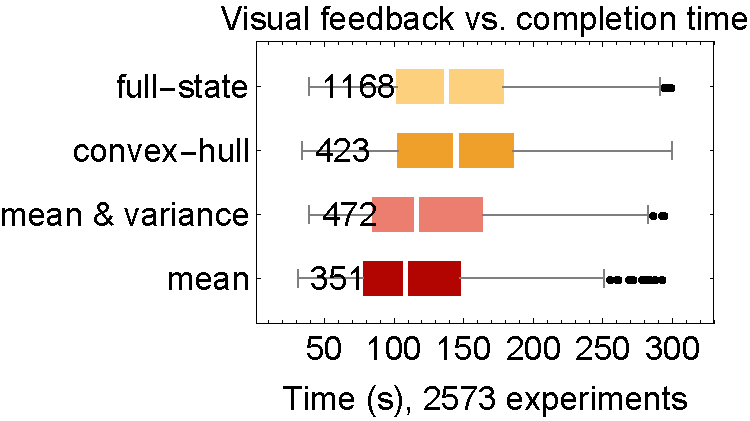
\includegraphics[width=0.5\textwidth]{ResVaryVis.pdf}
  \end{center}
  \vspace{-1em}
\caption{\label{fig:ResVaryVis} Completion-time results for the four levels of visual feedback shown in Fig.~\ref{fig:Visualization}.  Players performed better with limited feedback.
\vspace{-1em}
}
\end{wrapfigure}

Sensing is expensive, especially on the nanoscale. To see nanocars~\cite{Chiang2011} fastened molecules that fluoresce light when activated by a strong light source. Unfortunately, multiple exposures can destroy these molecules, a process called \emph{photobleaching}. Photobleaching can be minimized by lowering the excitation light intensity, but \cite{Cazes2001} showed this increases the probability of missed detections.  This experiment explores manipulation with varying amounts of sensing information: {\bf full-state} sensing provides the most information by showing the position of all robots; {\bf convex-hull} draws a convex hull around the outermost robots; {\bf mean} provides the average position of the population; and {\bf mean + variance} adds a confidence ellipse. Fig.~\ref{fig:Visualization} shows screenshots of the same robot swarm with each type of visual feedback. Full-state requires $2n$ data points for $n$ robots. Convex-hull requires at worst $2n$, but according to \cite{har2011expected}, the expected number is $O(2 n^{1/3})$.  Mean requires two, and variance three, data points.  Mean and mean + variance are convenient even with millions of robots. 

%\begin{figure}[b!]
%\renewcommand{\figwid}{0.5\columnwidth}
%\begin{overpic}[width =\figwid]{ResVaryVis.pdf}\end{overpic}
%\vspace{-1em}
%\caption{\label{fig:ResVaryVis} Completion-time results for the four levels of visual feedback shown in Fig.~\ref{fig:Visualization}.  Players performed better with limited feedback.
%%\vspace{-1em}
%}
%\end{figure}




% Additionally, as population characteristics, they are available even if only a percentage of the robots are detected each control cycle.
%Photobleaching: http://www.piercenet.com/browse.cfm?fldID=4DD9D52E-5056-8A76-4E6E-E217FAD0D86B
%
%Photobleaching is caused by the irreversible destruction of fluorophores due to either the prolonged exposure to the excitation source or exposure to high-intensity excitation light. Photobleaching can be minimized or avoided by exposing the fluor(s) to the lowest possible level of excitation light intensity for the shortest length of time that still yields the best signal detection; this requires optimization of the detection method using high sensitivity CCD cameras, high numerical aperture objective and/or the widest bandpass emission filter(s) available. Other approaches include using fluorophores that are more photostable than traditional fluorophores and/or using antifade reagents to protect the fluor(s) against photobleaching. Steps to avoid photobleaching are not feasible for all detection methods and should be optimized for each method used. For example, antifade reagents are toxic to live cells, and therefore they can only be used with fixed cells or tissue. Furthermore, some detection methods, such as flow cytometry, normally do not require steps to avoid photobleaching because of the extremely short exposure time of the fluorophore to the excitation source.


%\begin{figure}
%\centering
%\begin{overpic}[width = \columnwidth]{ResVaryVis.pdf}\end{overpic}
%\vspace{-2em}
%\caption{\label{fig:ResVaryVis} Completion-time results for the four levels of visual feedback shown in Fig.~\ref{fig:Visualization}. Surprisingly, players perform better with limited feedback--subjects with only the mean + variance  outperformed all others.
%\vspace{-2em}
%}
%\end{figure}

Our hypothesis predicted a steady decay in performance as the amount of visual feedback decreased.
Our experiment indicated the opposite: players with just the mean completed the task faster than those with full-state feedback.  As Fig.~\ref{fig:ResVaryVis}.b shows, the levels of feedback arranged by increasing completion time are [ mean, mean + variance, full-state, convex-hull].  All experiments lasting over 300s were removed, under the assumption that the user stopped playing. 
Using ANOVA analysis, we reject the null hypothesis that all visualization methods are equivalent, with $p$-value $2.69\times10^{-19}$.
Anecdotal evidence from beta-testers who played the game suggests that tracking 100 robots is overwhelming---similar to schooling phenomenons that confuse predators---while working with just the mean + variance is like using a ``spongy'' manipulator. Our beta-testers described convex-hull feedback as confusing and irritating.  A single robot left behind an obstacle will stretch the entire hull, obscuring the majority of the swarm.
%obscuring what the rest of the swarm is doing.   

\paragraph{Varying noise}
Microrobots are affected by random collisions with molecules. The effect of these collisions is called Brownian motion.

This experiment varied the strength of these disturbances to study how noise affects human control of large swarms. Noise was applied at every timestep as follows:
\begin{align*}
\dot{x}_i &= u_x + m_i\cos(\psi_i)\\
 \dot{y}_i &= u_y + m_i\sin(\psi_i).
 \end{align*}
$m_i,\psi_i$ are uniformly IID, with $m_i\in[0,M]$ and $\psi_i\in[0,2\pi]$. $M$ is a constant for each trial ranging from 0 to 200\% of the maximum control power ($u_{max}$).
 
We hypothesized 200\% noise was the largest a human could be expected to control---at 200\% noise, the robots move erratically.  Disproving our hypothesis, the results in Fig.~\ref{fig:ResVaryNoisePosition}.a show only a 40\% increase in completion time for the maximum noise.

\begin{figure}[b!]
\renewcommand{\figwid}{0.5\columnwidth}
\begin{overpic}[width =\figwid]{ResVaryNoise.pdf}\end{overpic}
\begin{overpic}[width =\figwid]{ResPositioning.pdf}\end{overpic}
\vspace{-1em}
\caption{\label{fig:ResVaryNoisePosition} Left: Varying the noise from 0 to 200\% of the maximum control input resulted in only a small increase in completion time. Right: Increasing the number of robots resulted in longer completion times.  For more than 4 robots the goal pattern contained a void, which may have caused the jump in completion times.
%\vspace{-1em}
}
\end{figure}


\paragraph{Position control}
This online experiment examined how completion time scales with the number of robots $n$. Using a single square obstacle, users arranged $n\in[1,10]$ robots into a specified goal pattern.  The goal pattern formed a block  {\sffamily A} with 10 robots, and lesser numbers of robots used a subset of these goal positions. Our hypothesis was that completion time would increase linearly with the number of robots, as with our position control algorithm in \cite{Becker2013b}.  Our results roughly corroborate this, as shown in Fig.~\ref{fig:ResVaryNoisePosition}.b.  Though the number of robots presented to game players is uniformly distributed, larger $n$ are more difficult, and the number of successful experiments drops steadily as $n$ increases.



Note there is a bifurcation between $n$=4 and $n$=5 robots. For $n\in[1,4]$ the goal patterns are not hollow, but starting at $n$=5 they are.  A better experiment design would randomly place the goal positions.  Initially we tried this, but our beta-testers strongly disliked trying to arrange robots in random patterns.


\paragraph{Varying control: Assembly}
Ultimately, we want to use swarms of robots to build things. This experiment compared different control architectures modeled after real-world devices.

We compared attractive and repulsive control with the global control used for the other experiments. The attractive and repulsive controllers were loosely modeled after scanning tunneling microscopes (STM), but also apply to magnetic manipulation, e.g.\ \cite{Khalil2013} and biological models, e.g. \cite{goodrich2012types}. STMs can be used to arrange atoms and make small assemblies, as described in \cite{avouris1995manipulation}. An STM tip is charged with electrical potential, and used to repel like-charged or to attract differently-charged molecules. In contrast, the global controller uses a uniform field (perhaps formed by parallel lines of differently-charged conductors) to pull molecules in the same direction.
The experiment challenged players to assemble a three-block pyramid with a swarm of 16 robots.

%\todo{describe controller model here, use an equation}

The results were conclusive, as shown in Fig.~\ref{fig:ResVaryControl}.a: attractive control was the fastest, followed by global control, with repulsive control a distant last.  The median time using repulsive control was four times longer than with attractive control.
Using ANOVA analysis, we reject the null hypothesis that all controllers are equivalent, with $p$-value $3.37\times10^{-32}$.

%%\begin{figure}
%%\begin{overpic}[width = 0.39\columnwidth]{attractiveForce.pdf}\end{overpic}
%%\begin{overpic}[width = 0.6\columnwidth]{understandingForces.pdf}\end{overpic}
%%\caption{
%%\label{fig:attractiveForce}
%%Attraction and repulsion with a point source distance $h$ above the plane and $r$ from the robot. 
%%}
%%\end{figure}

\begin{figure}[b!]
\renewcommand{\figwid}{3.3cm}
\begin{overpic}[height =\figwid]{ResVaryControl.pdf}\end{overpic}
\begin{overpic}[height =\figwid]{ResVaryForage.pdf}\end{overpic}
\vspace{-.5em}
\caption{\label{fig:ResVaryControl} Completion time depends on both the task and the control type. Left: Attractive control resulted in the shortest completion time and repulsive the longest for building a three-block pyramid. Right: in the foraging test, global control resulted in the shortest completion time and attractive the longest.
%\vspace{-1em}
}
\end{figure}

\paragraph{Varying control: Foraging}
Collecting and delivering resources is necessary for drug delivery.
This experiment also compared attractive and repulsive control with the global control used for the other experiments. The experiment challenged players to collect particles using a swarm of 100 robots and return the particles to a home region. The robots encapsulate the particles on contact. 

%\todo{describe controller model here, use an equation}

The results were conclusive, as shown in Fig.~\ref{fig:ResVaryControl}.b: global control was the fastest, followed by repulsive control, with attractive control last.  Using ANOVA analysis, we reject the null hypothesis that all controllers are equivalent, with $p$-value $2.96\times10^{-6}$.



%%%%%%%%%%%%%%%%%%%%%%%%%%%%%%%%%%%%%%%%%%%%%%%%%%%%%%%%%%%
%\section{Torque control}
%\label{sec:theory}
%%%%%%%%%%%%%%%%%%%%%%%%%%%%%%%%%%%%%%%%%%%%%%%%%%%%%%%%%%%
%\subsection{Controlling Torque}

%We derive inspiration from recent work on pulling with a swarm \cite{pulltogether}. The contribution of this work is to map swarm distributions to torque production.
%The orientation of an object's major axis is important when a swarm is manipulating a non-symmetric object through narrow corridors. 
%Orientation is controllable by applying torque to the object. 
%To change the output torque $\tau$ in~\eqref{eq:torque}, we can choose the direction and magnitude of the force applied $F$, and the moment arm from the object's center of mass (COM) $O$ to the point of contact $P$.
%We define a coordinate frame rooted at the COM, with the $x$-axis parallel to the object's longest axis. The resulting torque is:
%
%\begin{equation}
%\tau = F \times (P - O ).\label{eq:torque}
%\end{equation}
%
%We assume that the forces produced by individual particles add linearly. 
% As \cite{pulltogether} indicates, this is often a simplification of the true dynamics. 
% The swarm version of \eqref{eq:torque} is the summation of the forces contributed by $n$ individual particles:
%\begin{align}
%\tau_{\text{total}} &= \sum\limits_{i=1}^n \rho_i F_i \times (P_i - O ) \textrm{      and}   \label{eq:swarmtorque}\\
%F_{\text{total}} &= \sum\limits_{i=1}^n \rho_i F_i.  \label{eq:swarmforce}
%\end{align}
%Here $F_i$ is the force that the $i^{\textrm{th}}$ particle applies. 
%Not all particles are in contact with the object.  
%$\rho_i$ is an indicator variable: $\rho_i=1$ if the particle is in direct contact with the object or touching a chain of particle where at least one particle is in contact with the object. 
% Otherwise $\rho_i = 0$.
%The moment arm is the particle's position $P_i$ to the object's COM $O=[O_x,O_y]^{\top}$. 
% If all particles are identical and the control input is uniform, the force is equivalent for every particle and so $F_i $ equals some constant.
%

\section{Angle of repose}\label{sec:angle}




Consider a swarm of granular particles applying force to a rod. 
If the rod moves slower than the particles, these particles will build up behind the rod in a characteristic triangular shape defined by an apex angle. This piling up is common to all granular media, and the angle formed is a function of the \emph{angle of repose}. Three different values of angle of repose is shown in Fig.~\ref{fig:angle}. The center of mass of the rod is in the middle of the rod, but center of mass of the granular particles changes for different values of angle of repose. % for the media, see \cite{angleofRepose}. 
 By measuring the angle of repose for the particles shown in the top plot of Fig.~\ref{fig:AngleOfReposeForce}, we can estimate the force and torque that the swarm is applying to the rod as a function of the rod's length, the angle of repose, and orientation of the rod.
 We define the angle of repose as $\alpha$, the rod's orientation relative to 90$^\circ$ from the particle movement vector as $\theta$, and the rod's length as $\ell$. 
 \begin{figure}
\centering
\renewcommand{\figwid}{\columnwidth}
\begin{overpic}[width =\figwid]{Angle.pdf}%\put(1,55){a)}
\end{overpic}
\caption{\label{fig:angle} Different values of angle of repose is shown when granular particles move faster than the rod.
}
\end{figure}
By integrating over the triangular shape, the force applied to the rod (when a unit area of particles produces 1 N of force) is
\begin{figure}
\centering
\renewcommand{\figwid}{\columnwidth}
\begin{overpic}[width =0.6\figwid]{AngleOfRepose.pdf}%\put(1,55){a)}
\end{overpic}\\
\vspace{0.5em}
\begin{overpic}[width =0.6\figwid]{AngleOfReposeForce.pdf}%\put(1,55){a)}
\end{overpic}\\
\vspace{0.5em}
\begin{overpic}[width =0.6\figwid]{AngleOfReposeTorque.pdf}%\put(1,55){a)}
\end{overpic}
\vspace{-0.5em}
\caption{\label{fig:AngleOfReposeForce} Top plot shows colored particulate heaped up on pink-colored long rods. 
%Particulate is moving in the $-y$ direction, and the rods are tilted at $\theta=\{-45,-22.5,0,22.5,45\}^\circ$ with respect to the $x$ axis. 
% A thin gray line extends upwards from the rod COM, showing how more particulate is heaped on the right side of the rod for positive $\theta$ and more on the left side for negative $\theta$. 
%  This uneven particulate generates a restoring torque. 
 Middle plot shows the force applied to the rod and bottom the torque as a function of $\theta$ for four angle of repose values.
 %The rod length $\ell=1$. 
   The maximum torque values are shown with black dots.
% Generating code is in the attachment. 
%\vspace{-2em}
}
\end{figure}

\begin{align}
F(\theta,\alpha,\ell) =\left\{
\begin{array}{ll}
\frac{-\ell^2\Big(\cos(2\theta)-\cos(2\alpha)\Big)}{8\cos\alpha\sin{\theta}} &   -\alpha<\theta<\alpha\\
0 &    \textrm{otherwise .}\\
\end{array} 
\right .\\
\end{align}


%\begin{align}
%F(\theta,\alpha,l)  = \frac{l^2}{8\cos\alpha\sin{\theta}} \Big(\cos(2\theta)-\cos(2\alpha)\Big).
%\end{align}

The force for different angle of repose values are shown in the middle plot of Fig.~\ref{fig:AngleOfReposeForce}. 
Torque will also be similarly defined as
\begin{align}
\tau(\theta, \alpha, \ell) =\left\{
\begin{array}{ll}
\frac{\ell^3\Big(\cos(2\alpha)-\cos(2\theta)\Big)\sin{\theta} }{48\sin^2\alpha}&   -\alpha<\theta<\alpha\\
0 &    \textrm{otherwise .}\\
\end{array} 
\right.
\end{align}
Torque is shown in the bottom plot of Fig.~\ref{fig:AngleOfReposeForce}.
 Given sufficient particles to pile up to the angle of repose, this torque tends to stabilize the object to be perpendicular to the pushing direction.
Force is maximized with $\theta=0$, but the $\theta$ value that maximizes torque is a function of $\alpha$ and is defined as
\begin{align}
\theta_{t_{\max}} = \frac{\sin(\alpha)}{\sqrt{3}}.
\end{align}
To maximize the torque a particulate swarm applies on a thin rod, the swarm should move in the direction $-\theta_{t_{\max}} - 90^\circ$ with respect to the long axis of the rod.





\section{Simulation}\label{sec:simulation}


%Two simulations were implemented using non-slip contact walls for position control.  The first controls the position of two robots, the second controls the position of $n$ robots.  

%\subsection{Position Control of Two Robots}
\begin{figure}
\centering
\begin{overpic}[width=0.49\columnwidth]{worstnum.pdf}\put(0,75){a)}\end{overpic}
\begin{overpic}[width=0.49\columnwidth]{worstdist.pdf}\put(0,75){b)}\end{overpic}
\begin{overpic}[width=0.49\columnwidth]{middlegoalnum.pdf}\put(0,75){c)}\end{overpic}
\begin{overpic}[width=0.49\columnwidth]{middlegoaldist.pdf}\put(0,75){d)}\end{overpic}
\caption{\label{fig:contour}
Plots show performance with one goal on the boundary.
}
\end{figure}

\begin{figure}
\centering
%\begin{overpic}[width=\columnwidth]{deltanum.pdf}\end{overpic}\\
%\vspace{1em}
\begin{overpic}[width=\columnwidth]{deltadist.pdf}\end{overpic}
\vspace{-1em}
\caption{\label{fig:deltanumdist}
The worst case path length occurs when particles must swap antipodes. This can never be achieved but can be asymptotically approached. Plot shows decreasing error as the number of moves grows.
} 
\end{figure}


\begin{figure}
\centering
\renewcommand{\figwid}{1\columnwidth}
{
\begin{overpic}[width =\figwid]{contourDistnew.png}\put(-2,10){\begin{turn}{90} \tiny{unique particles}
\end{turn}}

\end{overpic}
\vspace{1em}
\begin{overpic}[width =\figwid]{JustSimulationV6.png}\put(-2,10){\begin{turn}{90} \tiny{unique particles}
\end{turn}}

\end{overpic}
\begin{overpic}[width =\figwid]{identical.png}\put(-2,6){\begin{turn}{90} \tiny{interchangeable particles}
\end{turn}}
\end{overpic}
}\caption{\label{fig:contourPlots}{Starting positions of particles $1$ and $2$ and goal position of particle $2$ are fixed, and $\epsilon=0.001$.
 The top row of contour plots show the distance if robot $1$'s goal position is varied in $x$ and $y$. The bottom row shows the number of moves required for the same configurations.}
\vspace{-1em}
}
\end{figure}
Algorithm \ref{alg:optimalAlg}  was implemented in Mathematica using particles with zero radius. 
%An online interactive demonstration and source code of the algorithm are available at \cite{Shahrokhi2015mathematicaParticle}.
%  Fig.~\ref{fig:shapeControlMathematica1}  shows  an implementation of this algorithm with robot initial positions represented by hollow squares and final positions by circles. 
 %Dashed lines show the shortest route if robots could be controlled independently, while solid lines show the optimal shortest  path using uniform inputs.
 
 The contour plots in Fig.~\ref{fig:contour} left show the length of the path for two different settings. Top row considers \{$s_1,s_2,g_1$\} = \{$(0.2,0.2),(-0.1,-0.1),(-0.2,0)$\} and bottom row considers  \{$s_1,s_2,g_1$\} = \{$(0.2,0.2),(-0.1,-0.1),(0,0)$\} in a workspace with $r= 0.5$, and $g_2$ ranging over all the workspace. Fig.~\ref{fig:contour} right shows the total distance of the path. This plot shows the nonlinear nature of the path planning. The path length grows when the goals have $\pi$ difference and are very close to the boundary. TODO:???? We need to discuss the new plots.
 The worst case occurs when the ending points are at antipodes along the boundary ($\pi$ angular distance). This can never be achieved but can be asymptotically approached as shown in Fig.~\ref{fig:deltanumdist}. 
 Fig.~\ref{fig:contourPlots} shows the same concepts in a square workspace. Fig.~\ref{fig:contourPlots} top and middle row considers the particles for three arbitrary starting and goal positions for the particles. All of the discussed plots have considered the particles to be unique. If particles are interchangeable and it does not matter to put the specific particle to its goal location, the path length will be significantly smaller. The bottom row of  Fig.~\ref{fig:contourPlots} considers interchangeable particles with the same configuration as the middle row with unique particles.
 
 %If the length of each side of the square workspace is $L$, the worst case path length is $(\sqrt{2}+2)L$.
 
% The plots in Fig.~\ref{fig:deltanumdist} show the exponentially increasing number of moves and distance when the accuracy of reaching to the goal ($\delta$) is getting to zero when the goal positions have $\pi$ difference with each on the boundaries.











%%%%%%%%%%%%%%%%%%%%%%%%%%%%%%%%%%%%%%%%%%%%%%%%%%%%%%%%%%%
\section{Experimental Results}\label{sec:expResults}
%%%%%%%%%%%%%%%%%%%%%%%%%%%%%%%%%%%%%%%%%%%%%%%%%%%%%%%%%%%
\begin{figure*}[htb!]\label{fig:3dPrinted}
\centering
\vspace{1.5em}
%\begin{overpic}[width=\columnwidth]{firstImage.jpg}\end{overpic}
\begin{overpic}[width=2\columnwidth]{3dexperiment.pdf}\end{overpic}
\\
\vspace{1em}
\begin{overpic}[width=2\columnwidth]{realTripe.pdf}\end{overpic}
\caption{\label{fig:story}
Frames showing particle positions before and after control inputs. Top row: small intestine phantom. Bottom row: cow stomach tissue.
} \vspace{-1em}
\end{figure*}

To demonstrate Alg.~\ref{alg:optimalAlg} experimentally, we performed several tests.
Each used the same magnetic setup shown in Fig.~\ref{fig:IntroPic}.
% The figure might need to be referenced 
 Two different intestine models were employed, the first a 3D-printed cross-section representation of a small intestine, and the second a cross-section of a bovine stomach.
 
 \subsection{Magnetic Manipulation Setup}
 
 The magnetic manipulation system has two pairs of electromagnetic coils, each with iron cores at their centers, and arranged orthogonal to each other. The iron core at the center of each coil concentrates the magnetic field towards the workspace. An Arduino and four SyRen regenerative motor drivers were used for control inputs to the coils. Finally, a FOculus F0134SB 659 x 494 pixel camera was attached to the top of the system, focusing on the workspace which was backlit by a $\SI{15}{\watt}$ LED light strip. 
 
To obtain experimental data, the test samples (the phantom intestine model and the bovine cross section) were placed in laser-cut acrylic discs and then immersed in corn syrup. Corn syrup was used to increase the viscosity to 12000 cP for the experiments. Spherical $\SI{1}{\milli\metre}$ magnets (supermagnetman \#SP0100-50) were used as our particles. Our experimental setup did not perfectly implement the system dynamics in \eqref{eq:swarmDynamicsAndFric}. In particular, the magnetic field in this setup is only approximately uniform. The magnetic force varies in both magnitude and orientation. As shown in the video attachment, this non-uniformity causes the particle closer to the coil to move faster than the other particle. This phenomenon makes it easier to increase particle separation than to decrease separation, but this can be compensated because boundary collisions easily decrease the separation. Also, magnetic forces are not exactly parallel, but point toward the center of the activated coil. Algorithm~\ref{alg:optimalAlg} still works despite these non-uniformities, but sometimes requires additional iterations.
 
%explain the magnetic field strength used, the camera system (briefly)
%explain the particles used

%explain the fluid used in the model.

\subsection{Intestine Phantom Model}

The intestine phantom model was used first and was made to mimic the geometry of an intestine and its villi. The model consists of a circular ring with an outer diameter of $\SI{50}{\milli\metre}$, an inner diameter of $\SI{46}{\milli\metre}$, and 60 $\SI{2}{\milli\metre}$ long protrusions on its inner surface cut out of $\SI{6}{\milli\metre}$ thick acrylic to model the geometry of intestinal villi. Figure \ref{fig:story} top row shows an experiment. Starting and ending positions were printed beneath the workspace on transparency film. Our algorithm successfully delivered the particles to goal positions in 10 out of 10 trials.

%methodology: we used xx material, built a model xx big


%todo: snapshots of the the beads in the model, moving toward goal.  We can add lots of annotations.  %Fake this series so we have an image for now.


\subsection{Bovine Stomach Cross-section}
%todo: procedure for fixating the Bovine tissue sample,
%discussion of the challenges 

Strips of cow stomach approximately $\SI{5}{\milli\metre}$ thick were cut and sewn to acrylic cylinder and then glued to an acrylic substrate using cyanoacrylate (superglue). This assembly was then filled with corn syrup. The experiment is shown in Fig.~\ref{fig:story} bottom row. Our algorithm successfully delivered the particles to goal positions in 5 out of 5 trials.
A video showing one trial of this experiment is available in the supplementary materials. 
%In using the small intestines, which were about 25mm in diameter, the resulting workspace was less than half of that of our simulated intestines. This meant more care had to be taken in navigating the magnets to their goal locations to avoid getting them too close to each other. 

%todo: snapshots of the the beads in the model, moving toward goal.  We can add lots of annotations.  Fake this series so we have an image for now.




%%%%%%%%%%%%%%%%%%%%%%%%%%%%%%%%%%%%%%%%%%%%%%%%%%%%%%%%%%%
\section{Object manipulation with hardware robots}\label{sec:realExperiment}
%%%%%%%%%%%%%%%%%%%%%%%%%%%%%%%%%%%%%%%%%%%%%%%%%%%%%%%%%%%
Our experiments use centimeter-scale hardware systems called \emph{kilobots}.  While those are far larger than the micro scale devices we model, using kilobots allows us to emulate a variety of dynamics, while enabling a high degree of control over robot function, the environment, and data collection. The kilobot, reported in \cite{Rubenstein2012,rubenstein2014programmable}, is a low-cost robot designed for testing collective algorithms with large numbers of robots. It is available commercially or as an open source platform from \cite{K-Team2015}.  Each robot is approximately 3 cm in diameter, 3 cm tall, and uses two vibration motors to move on a flat surface at speeds up to 1 cm/s.  Each robot has one ambient light sensor that is used to implement \emph{phototaxis},  moving towards a light source. 

  
\subsection{Environmental setup}  
In these experiments as shown in Fig.~\ref{fig:setup}, we used $n$=100 kilobots, a 1.5 m$\times$1.2 m whiteboard as the workspace, and lights: four 50W LED floodlights  at the corners and four 30W LED floodlights on the sides of a 6 m square centered on the workspace and 1.5 m above the table. The lights were controlled using an Arduino Uno board connected to an 8 relay shield board.  

Above the table, an overhead machine vision system tracks the swarm. The vision system identifies obstacles by color segmentation, determines the corners  (used to decrease  variance)  by topology, the object by color segmentation, and identifies robots using color segmentation and circle detection with a circular Hough transform.

The Laser-cut patterns for the neon green fiducial markers on the robots and {\sc Matlab} tracking code are available at our github repository~\cite{Shahrokhi2015GitHubShapeControl}. 
The objects were 3D printed from ABS plastic with a paper overlay. 
Shapes included a 325 cm$^2$ equilateral triangle, 
%Small Equilateral Triangle 140 cm$^2$,
 324 cm$^2$ square,
 281 cm$^2$ hexagon,
254 cm$^2$ circle, 
and a 486 cm$^2$ (18 cm$\times$27 cm)  rectangle.

\begin{figure*}
\begin{center}
	%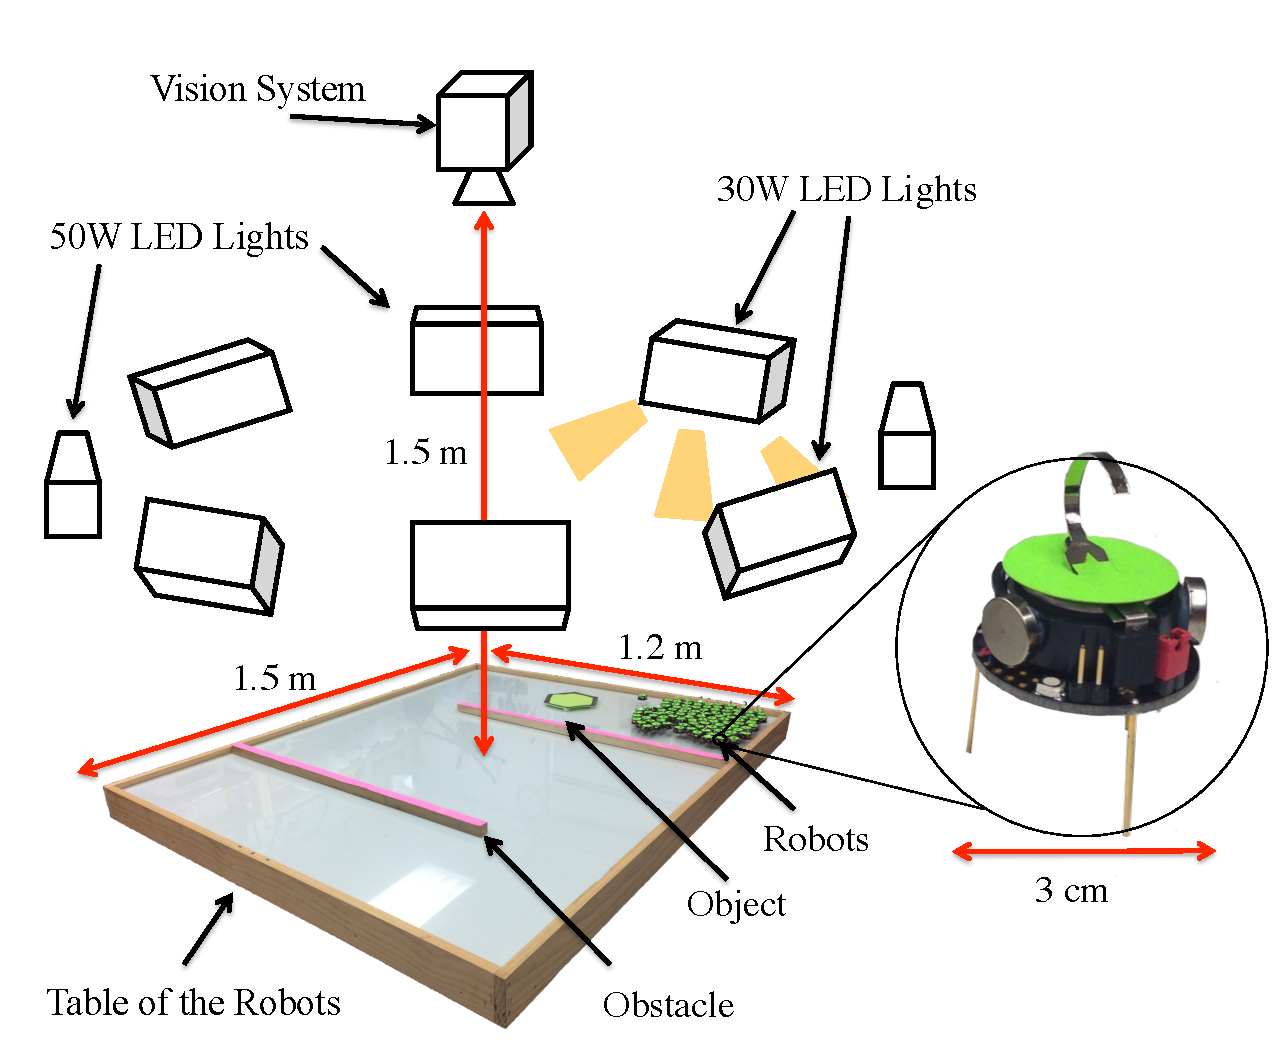
\includegraphics[width=0.5\columnwidth]{SetUp.pdf}
	\begin{overpic}[width=0.6\columnwidth]{SetUp.pdf}%\put(1,75){A}
	\end{overpic}\\
	\begin{overpic}[width=0.35\columnwidth]{AllShapesR.pdf}%\put(-0,85){B}
	\end{overpic}
	\begin{overpic}[width=0.35\columnwidth]{PotentialExp.pdf}%\put(-0,85){C}
	\end{overpic}
\end{center}

\caption{\label{fig:setup}
(Top) Hardware platform. (Lower left) Four shapes used for hardware experiments. (Lower right) Visualization of potential field. }
\end{figure*}

\paragraph{Swarm mean control (hardware experiment)}

Unlike the PD controller \eqref{eq:PDcontrolPosition}, we cannot command a force input to the kilobots.  Instead, control is given by turning on one of eight lights.  The kilobots run a phototaxis routine where they search for an orientation that aligns them with the light source, and then move with an approximately constant velocity toward this light.  In practice, because the kilobots only have one light detector, they oscillate along this orientation.  

We use the sign of \eqref{eq:PDcontrolPosition}, and choose the closest orientation among the eight light sources.
Fig.~\ref{fig:realMean} shows that this limited, discretized control still enables regulating the mean position of a swarm of 100 robots.


\begin{figure*}
\begin{center}
	\begin{overpic}[width=\columnwidth]{RealMean}\end{overpic}
%	\begin{overpic}[width=0.35\columnwidth]{XYMeanControl.eps}\end{overpic}
\end{center}
\vspace{-1em}
\caption{\label{fig:realMean}
Regulating average $x$ position of 100 kilobots using control law \eqref{eq:PDcontrolPosition}.
%Mean control plot with kilobots. %\todo{place a red star and a red circle at two spots on graph, put two images of the swar at right with a red star and red circle in left hand corner of these, and put a scale bar in image}
}
\end{figure*}

%\begin{figure}
%\begin{center}
%	\includegraphics[width=\columnwidth]{XYMeanControl.eps}
%\end{center}
%\caption{\label{fig:meanRobotFig}
%Mean Control experiment with kilobots.
%}
%\end{figure}

\subsection{Automated object manipulation (hardware experiment)}

The kilobots performed five successful runs of object manipulation through the obstacle maze.
Each trial used 100 kilobots. Videos of each are in the multimedia extension. Trials two-five were performed in a row with no failures in between.  For each trial, fully charged kilobots were placed in the lower left-hand of the workspace, as shown in Fig.~\ref{fig:expSnapShot}.  The moveable object was placed in the lower center of the workspace. The same controller as in the simulation, Alg.~\ref{alg:BlockPushing}, but with discretized control inputs, was coded in {\sc Matlab}.  Trials were run until the object COM entered the goal region.  The trials ran for \{24:25, 57:37, 50:00, 36:02, 45:07\} minutes.  This is a mean of 42:38 and a standard deviation of 12:51 minutes. 
A circular object completed in 52:35 minutes. 
A square object completed in 114:31 minutes. 
A triangular object completed in XX:YY minutes.

%Rules: http://www.ijrr.org/historic/MMVideoGuideLines.pdf



\begin{figure}
\centering
%\begin{overpic}[width=\columnwidth]{Snapshots.pdf}\put(6,29){\emph{t} = 3 s}\put(38,29){\emph{t} = 410 s}\put(70,29){\emph{t} = 710 s}
%\put(15,22){\emph{t} = 1374 s}\put(49,22){\emph{t} = 2185 s}\put(83,22){\emph{t} = 2703 s}
%\end{overpic}
\begin{overpic}[width=.9\columnwidth]{Snapshots.pdf}\put(6,80){\emph{t} = 3 s}\put(38,80){\emph{t} = 410 s}\put(70,80){\emph{t} = 710 s}
\put(15,8){\emph{t} = 1374 s}\put(49,8){\emph{t} = 2185 s}\put(83,8){\emph{t} = 2703 s}
\end{overpic}
\vspace{-1em}
\caption{\label{fig:expSnapShot}{Snapshots showing the object manipulation experiment with 100 kilobots under automatic control. The automatic controller classifies pink objects as obstacles and generates a policy to the goal. See the video attachment for an animation~\cite{ShivaVideo2015}}
%\vspace{-2em}
}
\end{figure}




%%%%%%%%%%%%%%%%%%%%%%%%%%%%%%%%%%%%%%%%%%%%%%%%%%%%%%%%%%%
\section{Conclusion and Future Work}\label{sec:conclusion}
%%%%%%%%%%%%%%%%%%%%%%%%%%%%%%%%%%%%%%%%%%%%%%%%%%%%%%%%%%%

This paper presented techniques for controlling the shape of a swarm of robots using uniform global inputs and interaction with boundary friction forces.  
The paper provided algorithms for precise position control, as well as robust and efficient covariance control. 
Extending algorithms \ref{alg:PosControl2Robots} and \ref{alg:PosControlNRobots}  to 3D is straightforward but increases the complexity.
Future efforts should be directed toward improving the technology and tailoring it to specific robot applications.

  With regard to technological advances, this includes designing controllers that efficiently regulate $\sigma_{xy}$, perhaps using Lyapunov-inspired controllers as in \citep{kim2015imparting}. 
 Additionally, this paper assumed nearly infinite wall friction.  The algorithms require retooling to handle small $\mu_f$ friction coefficients.  It may be possible to rank controllability as a function of friction.
%  In hardware, the wall friction can be varied by laser-cutting boundary walls with different of profiles. 
  
    

%TODO JOURNAL: design controllers that efficiently regulate $\sigma_{xy}$.
%TODO JOURNAL: We will design Lyapunov-inspired controllers for $\sigma_{xy}$ to prove controllability. 
%TODO JOURNAL:  and rank controllability as a function of friction.
% TODO: JOURNAL: and vary wall friction by laser-cutting boundary walls with a variety of profiles. 


%    Inspired by large-scale human experiments with swarms of robots under global control,  this paper investigated controllers that use only the mean and variance of a robot swarm. We proved that the mean position is controllable, and provided conditions under which variance is controllable.  We derived automatic controllers for each and a hysteresis-based switching control that controls the mean and variance of a robot swarm.  We employed these controllers as primitives for a block-pushing task. 
%    
%    Future work should implement these controllers on a robot swarm and decrease completion time by avoiding counter-productive contact with the block while the swarm is lowering its variance.  We have also assumed the swarm is unimodal and has a straight-line path to the moveable block. Relaxing these assumptions requires solving the \emph{gathering problem}.  The gathering problem for a swarm with uniform inputs is largely unexplored, and must be examined probabilistically for nontrivial environments.
%    
    % We should also control the covariance $\sigma_xy$ and higher moments of the distribution
    
    
    
%Sensing is expensive, especially on the nanoscale. To see nanocars~\citep{Chiang2011}, scientists fasten molecules that fluoresce light when activated by a strong light source. Unfortunately, multiple exposures can destroy these molecules, a process called \emph{photobleaching}. Photobleaching can be minimized by lowering the excitation light intensity, but this increases the probability of missed detections~\citep{Cazes2001}. A control methodology based on statistics of the robot swarm rather than the actual position of each robot, allows relaxing demands on imagine systems, controllers robust to tracking errors, and a simpler methodology.  In this work we...
%


% Additionally, as population characteristics, they are available even if only a percentage of the robots are detected each control cycle.
%Photobleaching: http://www.piercenet.com/browse.cfm?fldID=4DD9D52E-5056-8A76-4E6E-E217FAD0D86B
%
%Photobleaching is caused by the irreversible destruction of fluorophores due to either the prolonged exposure to the excitation source or exposure to high-intensity excitation light. Photobleaching can be minimized or avoided by exposing the fluor(s) to the lowest possible level of excitation light intensity for the shortest length of time that still yields the best signal detection; this requires optimization of the detection method using high sensitivity CCD cameras, high numerical aperture objective and/or the widest bandpass emission filter(s) available. Other approaches include using fluorophores that are more photostable than traditional fluorophores and/or using antifade reagents to protect the fluor(s) against photobleaching. Steps to avoid photobleaching are not feasible for all detection methods and should be optimized for each method used. For example, antifade reagents are toxic to live cells, and therefore they can only be used with fixed cells or tissue. Furthermore, some detection methods, such as flow cytometry, normally do not require steps to avoid photobleaching because of the extremely short exposure time of the fluorophore to the excitation source.


%\begin{dci}
%The Authors declare that there is no conflict of interest.
%\end{dci}
%\begin{funding}
%%RULES: http://www.nsf.gov/pubs/policydocs/pappguide/nsf16001/aag_6.jsp
%This work was supported by the National Science Foundation under Grant No.\ 
%\href{http://nsf.gov/awardsearch/showAward?AWD_ID=1553063}{ [IIS-1553063]}.
%\end{funding}
%\newpage
%\begin{sm}
%\begin{itemize}
%\item Extension 1:  simulation video of the parameter sweeps in Fig.~\ref{fig:AutoVeryParam} with robot swarms manipulating objects.
%\item Extension 2: hardware experiment videos of object manipulation with a swarm of 100 kilobots.
%\end{itemize}
%\end{sm}

   
%\input{11-MultiMediaAppendix.tex}
   
\bibliographystyle{IEEEtran}
%\bibliographystyle{SageH}
\bibliography{IEEEabrv,SwarmControlJournal}


\end{document}
